\chapter{Introduction}\label{sec:intro}
In this thesis methods to improve the stability of the electron gun of the \gls{flute} accelerator are studied.

\Gls{flute} is a \gls{linac}-based accelerator test-facility and a \gls{thz} photon source that is currently under commission at the \gls{kit}. It aims to be a source of high field \gls{thz} pulses (up to \SI{1200}{\mega\volt\per\meter}) in the femtosecond range, provide a test facility for accelerator research and an injection device for \gls{cstart} (see \cite{SchaeferHaererPapash2019_1000091183}) in the future. \cite{Naknaimueang:2011zz}

The accelerator is designed for a final electron momentum of \SI{41}{\MeV\per c} and bunch charges of \SIrange{1}{3000}{\pico\coulomb} with lengths of \SIrange{1}{300}{\fs}. The bunches are emitted with a repetition frequency of up to \SI{10}{\hertz}. \cite{Malygin2018}

\autoref{fig:fluteEgun-flutePaper} shows the finished accelerator schematically. It consists of the low energy section, the \gls{linac}, the four-dipole bunch compressor and several diagnostic instruments.\\
Along with several diagnostic devices, the low energy section contains the electron gun that pre-accelerates electrons to \SI{7}{\MeV\per c}. The electrons are generated photo-electrically at the cathode inside the gun through stimulation with \gls{uv} radiation (\SI{270}{\nm}) generated by a Ti:Sa laser. After that a solenoid is used to focus the electron beam for injection into the \gls{linac} section. The \gls{linac}, a 156-cell travelling wave structure, is then used to accelerate the electrons to \SI{41}{\MeV\per c}. With a setup of four dipole magnets, the bunches are compressed longitudinally before the last dipole is used to generate \gls{csr} and \gls{cer} for \gls{thz} experiments. \cite{Nasse:IPAC13-WEPWA010}

At the time of writing, the low energy section is fully operational and at the end, a Faraday cup is installed as a beam dump to measure the electron bunch charges. It has to be removed when the \gls{linac} section is commissioned.

\begin{figure}[tb]
	\centering
	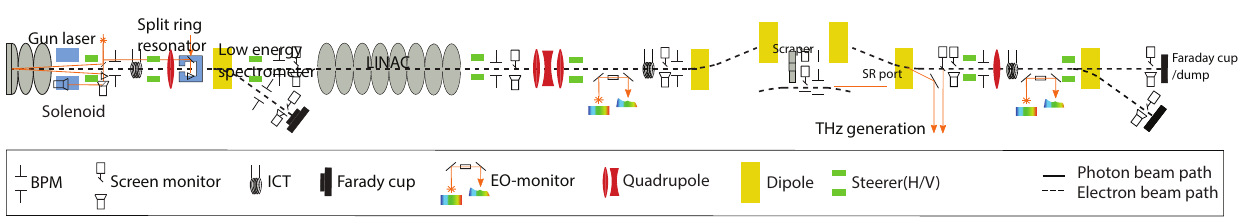
\includegraphics[width=\textwidth]{chap/StabilityOfTheElectronGun/img/flutePaper.png}
	\caption[FLUTE schematic with all components]{Schematic of the finished accelerator showing all installed and planned components (reprinted from \cite{Yan2018})}
	\label{fig:fluteEgun-flutePaper}
\end{figure}

Scientific experiments, such as \gls{thz} spectroscopy or the study of \gls{thz} radiation effects on biological tissue, rely on a known and stable wavelength of the \gls{thz} radiation. 

The \gls{thz} pulses used for experiments is mostly \gls{ctr}. This type of radiation is emitted when the short electron bunches interact with the vacuum-metalfoil interface at the screen downstream of the compressor section (see \autoref{fig:fluteEgun-flutePaper}). \cite{Yan:IPAC2016-WEPOY037,Thongbai2007}

According to \cite{ding2019coherent}, the energy spectrum of the \gls{ctr} emitted by a single electron (per frequency $\omega$ and solid angle $\Omega$) is given
\begin{equation}
\frac{\d{\xi}}{\d{\omega}\d{\Omega}} = \frac{q^2}{\pi^2 c} \left|S(\beta,\varphi,\phi)\right|^2
\end{equation}
with the electron charge $q$, the speed of light $c$, the angle $\varphi$ between the electron beam and the incidence plane, the angle $\phi$ between the incidence plane and the observation direction, the normalized electron velocity $\beta$ and
\begin{equation}
S(\beta,\varphi,\phi) = \frac{\beta \cos \varphi (\sin \phi -\beta \sin \varphi)}{(1-\beta \sin \phi \sin \varphi)^2-(\beta \cos \phi \cos \varphi)^2}.
\end{equation}
Therefore, the energy or the wavelength of the generated \gls{thz} photons depend on the electron velocity. The spread in \gls{thz} photon energy is thereby also a function of the electron velocity, so ultimately the electron energy.

Also, \gls{flute} being a test facility, adding and changing out components, possibly developed by other research institutes, is a common routine. To ensure compatibility among these components, reliable beam parameters at the interfaces between them are necessary. These parameters include the beams position in the horizontal and vertical direction, the beam steering angle, the electron energy, the emittance and the charge of the bunch and its dimensions. Since focusing and steering of the beam is done with electromagnets, it is also effected by the electron energy, as the deflection of an electron in a magnetic field is a function of its velocity, so ultimately its energy.

Besides depending on the wavelength of the \gls{uv} pulses hitting the cathode, the electron energies also strongly dependent of the  on the geometrical, electrical and thermal characteristics from the electron gun and its \gls{rf} power supply. These characteristics are not independent from each other and variations of them can have a multitude of intrinsic or extrinsic causes.

To improve the stability of the electron energy, in this thesis these causes are analyzed and measures against them or their effects are developed. Eventually this leads to the design of a \textit{closed}-loop control system. 

This approach is different from past efforts to improve the stability, which primarily treated the stability of (sub-) components that supply the electron gun. For instance, instabilities due to temperature variations were dealt with by stabilizing the water cooling system of the electron gun, or disturbances from the pulse forming network were reduced by improving the power supply. These measures can be thought of changes to an \textit{open}-loop. This is because there is no feeding back of the success or error from the system output, the electron energy, to the water cooler or power supply. Hence for these improvements to work, deep knowledge of the relation between the components and their effect on the electron energy is required. Also, if parameters of the components change due to aging, environmental factors, such as temperature or noise on the mains power, these effects can be carried over to the electron energy.

These are the main two reasons which motivate a closed-loop approach. It is often not required to know the exact relationships between certain input disturbances and the electron energy. Most of the times qualitative descriptions or correlations are sufficient, at least as a starting point, to achieve sufficiently good rejection of the disturbances. And with a closed-loop the system can react to changes of system parameters without the need for manual modifications.

That is why in the following chapter such a closed-loop control system for the \gls{flute} electron gun is treated in detail. In order to design an appropriate control system, some prerequisites are needed. First, the present disturbances are analyzed and metrics to later measure the favorable effect of the control system are defined. Then, ways of connecting the finished control system to the existing hard- and software are shown. With this preliminary work done, the control system can be designed. After the design process, the whole system is simulated on a computer to verify the solution, before the control system is implemented and tested with the real hardware, i.e. at \gls{flute}.

